\documentclass[]{article}
\usepackage{lmodern}
\usepackage{amssymb,amsmath}
\usepackage{ifxetex,ifluatex}
\usepackage{fixltx2e} % provides \textsubscript
\ifnum 0\ifxetex 1\fi\ifluatex 1\fi=0 % if pdftex
  \usepackage[T1]{fontenc}
  \usepackage[utf8]{inputenc}
\else % if luatex or xelatex
  \ifxetex
    \usepackage{mathspec}
  \else
    \usepackage{fontspec}
  \fi
  \defaultfontfeatures{Ligatures=TeX,Scale=MatchLowercase}
\fi
% use upquote if available, for straight quotes in verbatim environments
\IfFileExists{upquote.sty}{\usepackage{upquote}}{}
% use microtype if available
\IfFileExists{microtype.sty}{%
\usepackage{microtype}
\UseMicrotypeSet[protrusion]{basicmath} % disable protrusion for tt fonts
}{}
\usepackage[margin=1in]{geometry}
\usepackage{hyperref}
\PassOptionsToPackage{usenames,dvipsnames}{color} % color is loaded by hyperref
\hypersetup{unicode=true,
            pdftitle={Basic inferential data analysis of ToothGrowth dataset},
            pdfauthor={Thomas Fischer},
            colorlinks=true,
            linkcolor=blue,
            citecolor=Blue,
            urlcolor=Blue,
            breaklinks=true}
\urlstyle{same}  % don't use monospace font for urls
\usepackage{color}
\usepackage{fancyvrb}
\newcommand{\VerbBar}{|}
\newcommand{\VERB}{\Verb[commandchars=\\\{\}]}
\DefineVerbatimEnvironment{Highlighting}{Verbatim}{commandchars=\\\{\}}
% Add ',fontsize=\small' for more characters per line
\usepackage{framed}
\definecolor{shadecolor}{RGB}{248,248,248}
\newenvironment{Shaded}{\begin{snugshade}}{\end{snugshade}}
\newcommand{\KeywordTok}[1]{\textcolor[rgb]{0.13,0.29,0.53}{\textbf{#1}}}
\newcommand{\DataTypeTok}[1]{\textcolor[rgb]{0.13,0.29,0.53}{#1}}
\newcommand{\DecValTok}[1]{\textcolor[rgb]{0.00,0.00,0.81}{#1}}
\newcommand{\BaseNTok}[1]{\textcolor[rgb]{0.00,0.00,0.81}{#1}}
\newcommand{\FloatTok}[1]{\textcolor[rgb]{0.00,0.00,0.81}{#1}}
\newcommand{\ConstantTok}[1]{\textcolor[rgb]{0.00,0.00,0.00}{#1}}
\newcommand{\CharTok}[1]{\textcolor[rgb]{0.31,0.60,0.02}{#1}}
\newcommand{\SpecialCharTok}[1]{\textcolor[rgb]{0.00,0.00,0.00}{#1}}
\newcommand{\StringTok}[1]{\textcolor[rgb]{0.31,0.60,0.02}{#1}}
\newcommand{\VerbatimStringTok}[1]{\textcolor[rgb]{0.31,0.60,0.02}{#1}}
\newcommand{\SpecialStringTok}[1]{\textcolor[rgb]{0.31,0.60,0.02}{#1}}
\newcommand{\ImportTok}[1]{#1}
\newcommand{\CommentTok}[1]{\textcolor[rgb]{0.56,0.35,0.01}{\textit{#1}}}
\newcommand{\DocumentationTok}[1]{\textcolor[rgb]{0.56,0.35,0.01}{\textbf{\textit{#1}}}}
\newcommand{\AnnotationTok}[1]{\textcolor[rgb]{0.56,0.35,0.01}{\textbf{\textit{#1}}}}
\newcommand{\CommentVarTok}[1]{\textcolor[rgb]{0.56,0.35,0.01}{\textbf{\textit{#1}}}}
\newcommand{\OtherTok}[1]{\textcolor[rgb]{0.56,0.35,0.01}{#1}}
\newcommand{\FunctionTok}[1]{\textcolor[rgb]{0.00,0.00,0.00}{#1}}
\newcommand{\VariableTok}[1]{\textcolor[rgb]{0.00,0.00,0.00}{#1}}
\newcommand{\ControlFlowTok}[1]{\textcolor[rgb]{0.13,0.29,0.53}{\textbf{#1}}}
\newcommand{\OperatorTok}[1]{\textcolor[rgb]{0.81,0.36,0.00}{\textbf{#1}}}
\newcommand{\BuiltInTok}[1]{#1}
\newcommand{\ExtensionTok}[1]{#1}
\newcommand{\PreprocessorTok}[1]{\textcolor[rgb]{0.56,0.35,0.01}{\textit{#1}}}
\newcommand{\AttributeTok}[1]{\textcolor[rgb]{0.77,0.63,0.00}{#1}}
\newcommand{\RegionMarkerTok}[1]{#1}
\newcommand{\InformationTok}[1]{\textcolor[rgb]{0.56,0.35,0.01}{\textbf{\textit{#1}}}}
\newcommand{\WarningTok}[1]{\textcolor[rgb]{0.56,0.35,0.01}{\textbf{\textit{#1}}}}
\newcommand{\AlertTok}[1]{\textcolor[rgb]{0.94,0.16,0.16}{#1}}
\newcommand{\ErrorTok}[1]{\textcolor[rgb]{0.64,0.00,0.00}{\textbf{#1}}}
\newcommand{\NormalTok}[1]{#1}
\usepackage{graphicx,grffile}
\makeatletter
\def\maxwidth{\ifdim\Gin@nat@width>\linewidth\linewidth\else\Gin@nat@width\fi}
\def\maxheight{\ifdim\Gin@nat@height>\textheight\textheight\else\Gin@nat@height\fi}
\makeatother
% Scale images if necessary, so that they will not overflow the page
% margins by default, and it is still possible to overwrite the defaults
% using explicit options in \includegraphics[width, height, ...]{}
\setkeys{Gin}{width=\maxwidth,height=\maxheight,keepaspectratio}
\IfFileExists{parskip.sty}{%
\usepackage{parskip}
}{% else
\setlength{\parindent}{0pt}
\setlength{\parskip}{6pt plus 2pt minus 1pt}
}
\setlength{\emergencystretch}{3em}  % prevent overfull lines
\providecommand{\tightlist}{%
  \setlength{\itemsep}{0pt}\setlength{\parskip}{0pt}}
\setcounter{secnumdepth}{0}
% Redefines (sub)paragraphs to behave more like sections
\ifx\paragraph\undefined\else
\let\oldparagraph\paragraph
\renewcommand{\paragraph}[1]{\oldparagraph{#1}\mbox{}}
\fi
\ifx\subparagraph\undefined\else
\let\oldsubparagraph\subparagraph
\renewcommand{\subparagraph}[1]{\oldsubparagraph{#1}\mbox{}}
\fi

%%% Use protect on footnotes to avoid problems with footnotes in titles
\let\rmarkdownfootnote\footnote%
\def\footnote{\protect\rmarkdownfootnote}

%%% Change title format to be more compact
\usepackage{titling}

% Create subtitle command for use in maketitle
\newcommand{\subtitle}[1]{
  \posttitle{
    \begin{center}\large#1\end{center}
    }
}

\setlength{\droptitle}{-2em}
  \title{Basic inferential data analysis of ToothGrowth dataset}
  \pretitle{\vspace{\droptitle}\centering\huge}
  \posttitle{\par}
  \author{Thomas Fischer}
  \preauthor{\centering\large\emph}
  \postauthor{\par}
  \predate{\centering\large\emph}
  \postdate{\par}
  \date{May 30, 2018}

\usepackage{booktabs}
\usepackage{longtable}
\usepackage{array}
\usepackage{multirow}
\usepackage[table]{xcolor}
\usepackage{wrapfig}
\usepackage{float}
\usepackage{colortbl}
\usepackage{pdflscape}
\usepackage{tabu}
\usepackage{threeparttable}
\usepackage{threeparttablex}
\usepackage[normalem]{ulem}
\usepackage{makecell}

\begin{document}
\maketitle
\begin{abstract}
\textbf{\emph{This document provides the assignment `Course Project Part
2' for Coursera's Statistical Inference Class in the Coursera Data
Science series. Replication files are available on the author's Github
account (\url{https://github.com/tomfischersz}).}}
\end{abstract}

\section{1. Synopsis}\label{synopsis}

In this report we aim to conduct some basic inferential data analysis on
the ToothGrowth dataset of the R library `datasets'. We aim to answer
the question, if dosage and/or delivery method of vitamin C affects
tooth growth in guinea pigs. We therefore observe patterns from the
data, formulate hypotheses and then use statistical tests like confident
intervals or student's t-test to validate these hypotheses.

\section{2. The ToothGrowth Data Set}\label{the-toothgrowth-data-set}

The data consists of 60 observations with 3 variables, here the first
few observations: \rowcolors{2}{gray!6}{white}

\begin{table}[!h]

\caption{\label{tab:unnamed-chunk-9}The first few observations of the data set 
      ToothGrowth\label{tab:show_obs}}
\centering
\begin{tabular}[t]{rlr}
\hiderowcolors
\toprule
len & supp & dose\\
\midrule
\showrowcolors
4.2 & VC & 0.5\\
11.5 & VC & 0.5\\
7.3 & VC & 0.5\\
\bottomrule
\end{tabular}
\end{table}

\rowcolors{2}{white}{white}

The help page\footnote{Use R command help(ToothGrowth) to get further
  information.} for the data set ToothGrowth gives following
description:

\begin{quote}
The response is the length of odontoblasts (cells responsible for tooth
growth) in 60 guinea pigs. Each animal received one of three dose levels
of vitamin C (0.5, 1, and 2 mg/day) by one of two delivery methods,
(orange juice or ascorbic acid (a form of vitamin C and coded as VC).
\end{quote}

Our data are results from a study performed on guinea pigs to determine
the effect of vitamin C on tooth growth. The data contains 3 variables:

\begin{itemize}
\tightlist
\item
  \textbf{len:} The response (dependent) variable for the experiment
  measured for 60 guinea pigs is the tooth length.
\item
  \textbf{supp} and \textbf{dose} Two factors (independent variables),
  the delivery method of the vitamin C (supplement type) and the dose
  levels of vitamin C in mg/day. We are interested in the effect of
  these two factors on the response.
\end{itemize}

Table \ref{tab:data_summary} depicts a aggregated summary of our data.
We can see that there are 6 factor-level combinations and each of these
6 combinations were applied to 10 guinea pigs each. We hereafter call
this different combinations just treatment (and also added a new
column), e.g. ``OJ\_0.5'' just denotes the treatment with the factors
`Orange Juice' with a dose level of 0.5 mg/day.

\section{3.Exploratory Data Analysis}\label{exploratory-data-analysis}

We now visualize the means and spread of tooth growth for our six
distinct treatment groups (\protect\hyperlink{Appendix_1}{Code}):

\begin{figure}[h]

{\centering 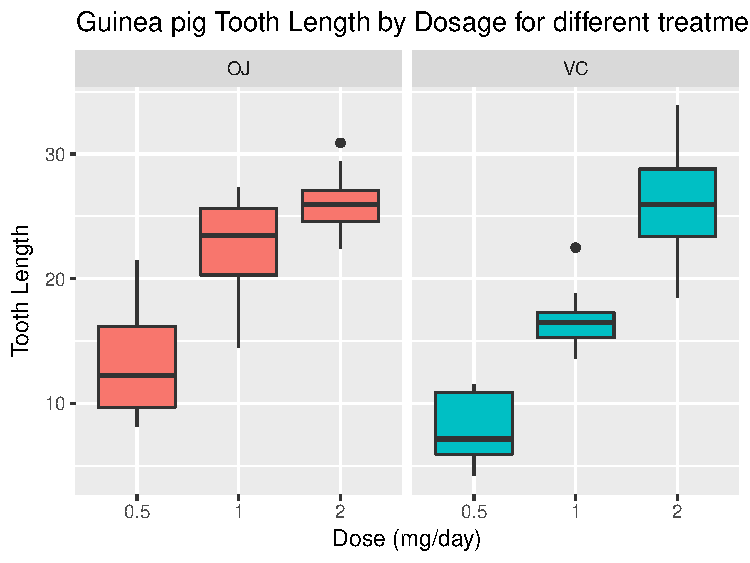
\includegraphics{toothgrowth_analysis_files/figure-latex/plot_fig_1-1} 

}

\caption{\label{fig:boxplot_1}Comparing the possible effects of three varying doses of vitamin C for the two different supplement types (Orange Juice and Vitamin C).}\label{fig:plot_fig_1}
\end{figure}

Figure \ref{fig:boxplot_1} suggests that the dose and the delivery
method both have some effect on the tooth growth. It appears that the
average tooth growth increases with the dose levels and that orange
juice might have higher growth rates than Vitamin C except for dose
levels of 2 mg.

\section{4. Basic Inference Analysis (hypothesis
tests)}\label{basic-inference-analysis-hypothesis-tests}

We are now testing several hypotheses. Our significance level (i.e.~the
risk of getting a Type I error) for all tests will be \(\alpha=0.05\).
We strictly only use student t-tests as required in the assignment
(disregarding regression analysis and anova test).

\subsection{4.1 Assumptions}\label{assumptions}

Before proceeding in our analysis it is important to assure certain
assumptions necessary to apply student's t-test, so we must be sure that
following assumptions are not violated:

\begin{itemize}
\item
  Independent and identically distributed: We are assuming that the
  process of choosing 60 guinea pigs for the experiment was independed
  and that they are drawn from the same population. Otherwise our
  results would be not reliable, e.g.~if the guinea pigs origin from two
  different breeders, or there are differences in male and female
  populations our conclusions could be flawed.
\item
  The probability distributions of the measured tooth length for each
  treatment are normal. Depicting Figure \ref{fig:fig_2} it seems that
  this assumption appears to be reasonably satisfied.
\end{itemize}

\subsection{4.2 Hypothesis Test I}\label{hypothesis-test-i}

We want to test the null hypothesis that the mean tooth length for the
two delivery methods are equal against the alternative hypothesis that
they differ:

\(H_0:\mu_{OJ}=\mu_{VC}\)\\
\(H_a:\mu_{OJ}\neq\mu_{VC}\)

Stated the relevant null and alternative hypotheses, we then conduct a
two-tailed t-test (\protect\hyperlink{Appendix_2}{Code}):

\begin{verbatim}
## 
##  Welch Two Sample t-test
## 
## data:  len by supp
## t = 1.9153, df = 55.309, p-value = 0.06063
## alternative hypothesis: true difference in means is not equal to 0
## 95 percent confidence interval:
##  -0.1710156  7.5710156
## sample estimates:
## mean in group OJ mean in group VC 
##         20.66333         16.96333
\end{verbatim}

As the obtained p-value of 0.061 is greater than the significance level
of 0.05 (and the confidence interval at 95\% contains 0) we cannot
reject our null hypothesis. Looking at figure \ref{fig:boxplot_1} again,
failing to reject the null hypothesis is likely due to the similar
results in tooth length for a vitamin C dose of 2 mg/day.

\subsection{4.2 Hypothesis Test II}\label{hypothesis-test-ii}

Our next hypothesis test will be examining if, for orange juice only,
higher doses of vitamin C are significantly associated with higher tooth
length. We are conducting two one-tailed t-tests and therefore need to
adjust our confidence intervals. We adjust the original confidence level
of our tests of 95\% using Bonferroni correction to
\(1-\frac{\alpha}{m}=0.975\), where \(m\) is the number of hypotheses.
Our new significance level is \(\alpha=0.025\).

\(H_0:\mu_{OJ\_0.5}=\mu_{OJ\_1}=\mu_{OJ\_2}\)\\
\(H_a:\) \(\mu_{OJ\_0.5}<=\mu_{OJ\_1}<=\mu_{OJ\_2}\)

Conducted the relevant t-test (\protect\hyperlink{Appendix_3}{Code}) we
get following results: \rowcolors{2}{gray!6}{white}

\begin{table}[!h]

\caption{\label{tab:print_sum_ttests}Summary of t-tests for different levels of doses (Orange Juice)\label{tab:sum_ttests}}
\centering
\begin{tabular}[t]{lrrr}
\hiderowcolors
\toprule
Sample Groups & p-values & Lower Conf.Interval & Upper Conf.Interval\\
\midrule
\showrowcolors
OJ\_0.5 versus OJ\_1 & 0.00 & -Inf & -5.52\\
OJ\_0.5 versus OJ\_1 & 0.02 & -Inf & -0.19\\
\bottomrule
\end{tabular}
\end{table}

\rowcolors{2}{white}{white}

As we can see, both p-values are below our significance level
\(\alpha=0.025\) and both confidence intervals for the difference of
means for the treatments are below zeros. We therefore can conclude to
reject the null hypothesis, i.e.~for orange juice we examine different
effects depending on the dose of vitamin C.

\subsection{5. Conclusion}\label{conclusion}

\begin{itemize}
\tightlist
\item
  No evidence for the hypothesis that tooth length differs for different
  delivery methods.
\item
  Strong evidence that tooth length varies for different doses given the
  delivery method orange juice.
\end{itemize}

\newpage

\section{Appendix I: Figures and
Tables}\label{appendix-i-figures-and-tables}

\rowcolors{2}{gray!6}{white}

\begin{table}[!h]

\caption{\label{tab:show_df_summary}Summary of the different treatments for the guinea pigs with
      their associated average tooth length and the corresponding standard
      deviation\label{tab:data_summary}}
\centering
\begin{tabular}[t]{lrlrrr}
\hiderowcolors
\toprule
Supplement & Dose (mg/day) & Treatment & N (number of pigs) & Mean & Standard Deviation\\
\midrule
\showrowcolors
OJ & 0.5 & OJ\_0.5 & 10 & 13.23 & 4.46\\
OJ & 1.0 & OJ\_1 & 10 & 22.70 & 3.91\\
OJ & 2.0 & OJ\_2 & 10 & 26.06 & 2.66\\
VC & 0.5 & VC\_0.5 & 10 & 7.98 & 2.75\\
VC & 1.0 & VC\_1 & 10 & 16.77 & 2.52\\
VC & 2.0 & VC\_2 & 10 & 26.14 & 4.80\\
\bottomrule
\end{tabular}
\end{table}

\rowcolors{2}{white}{white}

\begin{figure}[h]

{\centering 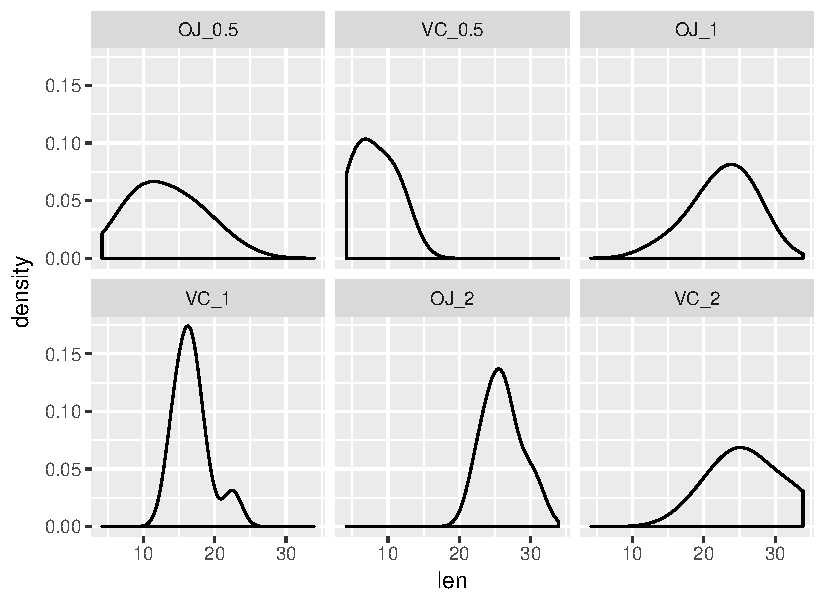
\includegraphics{toothgrowth_analysis_files/figure-latex/plot_fig_2-1} 

}

\caption{\label{fig:fig_2}Density distributions for all treatment groups.}\label{fig:plot_fig_2}
\end{figure}

\section{Appendix II: R Source Code}\label{appendix-ii-r-source-code}

\subsubsection{1. Load required
libraries:}\label{load-required-libraries}

\begin{Shaded}
\begin{Highlighting}[]
\KeywordTok{require}\NormalTok{(knitr)}
\KeywordTok{require}\NormalTok{(kableExtra)}
\KeywordTok{require}\NormalTok{(datasets)}
\KeywordTok{require}\NormalTok{(ggplot2)}
\KeywordTok{require}\NormalTok{(dplyr)}
\end{Highlighting}
\end{Shaded}

\subsubsection{2. Load data:}\label{load-data}

\begin{Shaded}
\begin{Highlighting}[]
\KeywordTok{data}\NormalTok{(ToothGrowth)}
\CommentTok{# names(ToothGrowth) <- c('length', 'supplement', 'dose')}
\end{Highlighting}
\end{Shaded}

\subsubsection{3. Add new variable
treatment:}\label{add-new-variable-treatment}

\begin{Shaded}
\begin{Highlighting}[]
\NormalTok{ToothGrowth}\OperatorTok{$}\NormalTok{treatment=}\KeywordTok{with}\NormalTok{(ToothGrowth,}\KeywordTok{interaction}\NormalTok{(supp,dose, }\DataTypeTok{sep =} \StringTok{'_'}\NormalTok{))}
\end{Highlighting}
\end{Shaded}

\subsubsection{4. First few observations:}\label{first-few-observations}

\begin{Shaded}
\begin{Highlighting}[]
\KeywordTok{kable}\NormalTok{(}\KeywordTok{head}\NormalTok{(ToothGrowth[, }\DecValTok{1}\OperatorTok{:}\DecValTok{3}\NormalTok{], }\DataTypeTok{n=}\DecValTok{3}\NormalTok{),}
      \DataTypeTok{format =} \StringTok{'latex'}\NormalTok{,}
      \DataTypeTok{booktabs =} \OtherTok{TRUE}\NormalTok{,}
      \DataTypeTok{caption =} \StringTok{"The first few observations of the data set }
\StringTok{      ToothGrowth}\CharTok{\textbackslash{}\textbackslash{}}\StringTok{label\{tab:show_obs\}"}\NormalTok{)  }\OperatorTok
\StringTok{    }\KeywordTok{kable_styling}\NormalTok{(}\DataTypeTok{latex_options =} \KeywordTok{c}\NormalTok{(}\StringTok{"striped"}\NormalTok{, }\StringTok{"hold_position"}\NormalTok{))}
\end{Highlighting}
\end{Shaded}

\subsubsection{5. Aggregating data in
data.frame:}\label{aggregating-data-in-data.frame}

\begin{Shaded}
\begin{Highlighting}[]
\NormalTok{df_summary <-}
\StringTok{    }\NormalTok{ToothGrowth }\OperatorTok
\StringTok{    }\KeywordTok{group_by}\NormalTok{(supp, dose, treatment) }\OperatorTok
\StringTok{    }\KeywordTok{summarise}\NormalTok{(}\DataTypeTok{N =} \KeywordTok{n}\NormalTok{(),}
              \DataTypeTok{mean_len =} \KeywordTok{mean}\NormalTok{(len),}
              \DataTypeTok{sd_len =} \KeywordTok{sd}\NormalTok{(len)) }\OperatorTok
\StringTok{    }\KeywordTok{as.data.frame}\NormalTok{()}
\end{Highlighting}
\end{Shaded}

\hypertarget{Appendix_1}{\subsubsection{6. Boxplots for different
treatments:}\label{Appendix_1}}

\begin{Shaded}
\begin{Highlighting}[]
\NormalTok{fig_}\DecValTok{1}\NormalTok{ <-}\StringTok{ }\KeywordTok{ggplot}\NormalTok{(ToothGrowth, }\KeywordTok{aes}\NormalTok{(}\DataTypeTok{x=}\KeywordTok{factor}\NormalTok{(dose), }\DataTypeTok{y=}\NormalTok{len)) }\OperatorTok{+}
\StringTok{    }\KeywordTok{facet_grid}\NormalTok{(.}\OperatorTok{~}\NormalTok{supp) }\OperatorTok{+}
\StringTok{    }\KeywordTok{geom_boxplot}\NormalTok{(}\KeywordTok{aes}\NormalTok{(}\DataTypeTok{fill =}\NormalTok{ supp), }\DataTypeTok{show.legend =} \OtherTok{FALSE}\NormalTok{) }\OperatorTok{+}
\StringTok{    }\KeywordTok{labs}\NormalTok{(}\DataTypeTok{title =} \StringTok{"Guinea pig Tooth Length by Dosage for different treatments"}\NormalTok{, }
         \DataTypeTok{x =} \StringTok{"Dose (mg/day)"}\NormalTok{,}
         \DataTypeTok{y =} \StringTok{"Tooth Length"}\NormalTok{)}
\end{Highlighting}
\end{Shaded}

\subsubsection{7. Distribution of Tooth Length for different
treatments:}\label{distribution-of-tooth-length-for-different-treatments}

\begin{Shaded}
\begin{Highlighting}[]
\NormalTok{fig_}\DecValTok{2}\NormalTok{ <-}\StringTok{ }\KeywordTok{ggplot}\NormalTok{(ToothGrowth, }\KeywordTok{aes}\NormalTok{(}\DataTypeTok{x =}\NormalTok{ len)) }\OperatorTok{+}
\StringTok{    }\KeywordTok{geom_density}\NormalTok{(}\DataTypeTok{adjust =} \FloatTok{1.5}\NormalTok{) }\OperatorTok{+}\StringTok{ }
\StringTok{    }\KeywordTok{facet_wrap}\NormalTok{(}\OperatorTok{~}\StringTok{ }\NormalTok{treatment)}
\end{Highlighting}
\end{Shaded}

\hypertarget{Appendix_2}{\subsubsection{8. Hypothesis Test
I}\label{Appendix_2}}

\begin{Shaded}
\begin{Highlighting}[]
\NormalTok{t_}\DecValTok{01}\NormalTok{ <-}\StringTok{ }\KeywordTok{t.test}\NormalTok{(len}\OperatorTok{~}\NormalTok{supp,}\DataTypeTok{data=}\NormalTok{ToothGrowth, }\DataTypeTok{paired =} \OtherTok{FALSE}\NormalTok{, }\DataTypeTok{var.equal =} \OtherTok{FALSE}\NormalTok{, }\DataTypeTok{alternative =} \StringTok{'two.sided'}\NormalTok{)}
\end{Highlighting}
\end{Shaded}

\hypertarget{Appendix_3}{\subsubsection{9. Hypothesis Test
II}\label{Appendix_3}}

\begin{Shaded}
\begin{Highlighting}[]
\NormalTok{t_02_}\DecValTok{1}\NormalTok{ <-}
\StringTok{    }\KeywordTok{t.test}\NormalTok{(len}\OperatorTok{~}\NormalTok{dose,}
           \DataTypeTok{data =}\NormalTok{ ToothGrowth[ToothGrowth}\OperatorTok{$}\NormalTok{treatment }\OperatorTok\StringTok{ }\KeywordTok{c}\NormalTok{(}\StringTok{'OJ_0.5'}\NormalTok{, }\StringTok{'OJ_1'}\NormalTok{),],}
           \DataTypeTok{paired =} \OtherTok{FALSE}\NormalTok{, }\DataTypeTok{var.equal =} \OtherTok{FALSE}\NormalTok{,}
           \DataTypeTok{alternative =} \StringTok{'less'}\NormalTok{, }\DataTypeTok{conf.level =} \FloatTok{0.975}\NormalTok{)}
\NormalTok{t_02_}\DecValTok{2}\NormalTok{ <-}
\StringTok{    }\KeywordTok{t.test}\NormalTok{(len}\OperatorTok{~}\NormalTok{dose,}
           \DataTypeTok{data =}\NormalTok{ ToothGrowth[ToothGrowth}\OperatorTok{$}\NormalTok{treatment }\OperatorTok\StringTok{ }\KeywordTok{c}\NormalTok{(}\StringTok{'OJ_1'}\NormalTok{, }\StringTok{'OJ_2'}\NormalTok{),],}
           \DataTypeTok{paired =} \OtherTok{FALSE}\NormalTok{, }\DataTypeTok{var.equal =} \OtherTok{FALSE}\NormalTok{,}
           \DataTypeTok{alternative =} \StringTok{'less'}\NormalTok{, }\DataTypeTok{conf.level =} \FloatTok{0.975}\NormalTok{)}
\NormalTok{sum_ttests <-}
\StringTok{    }\KeywordTok{data.frame}\NormalTok{(}\DataTypeTok{sample_group =} \KeywordTok{c}\NormalTok{(}\StringTok{'OJ_0.5 versus OJ_1'}\NormalTok{, }\StringTok{'OJ_0.5 versus OJ_1'}\NormalTok{),}
               \DataTypeTok{p_value =} \KeywordTok{c}\NormalTok{(}\KeywordTok{round}\NormalTok{(t_02_}\DecValTok{1}\OperatorTok{$}\NormalTok{p.value,}\DecValTok{4}\NormalTok{), }\KeywordTok{round}\NormalTok{(t_02_}\DecValTok{2}\OperatorTok{$}\NormalTok{p.value,}\DecValTok{4}\NormalTok{)),}
               \DataTypeTok{confint_lower =} \KeywordTok{c}\NormalTok{(t_02_}\DecValTok{1}\OperatorTok{$}\NormalTok{conf.int[[}\DecValTok{1}\NormalTok{]], t_02_}\DecValTok{2}\OperatorTok{$}\NormalTok{conf.int[[}\DecValTok{1}\NormalTok{]]),}
               \DataTypeTok{confint_upper =} \KeywordTok{c}\NormalTok{(t_02_}\DecValTok{1}\OperatorTok{$}\NormalTok{conf.int[[}\DecValTok{2}\NormalTok{]], t_02_}\DecValTok{2}\OperatorTok{$}\NormalTok{conf.int[[}\DecValTok{2}\NormalTok{]]))}
\end{Highlighting}
\end{Shaded}


\end{document}
